\chapter{Diagramas de Bruijn}
Los diagramas de Bruijn fueron originalmente propuestos en teoría de registro de desplazamiento \cite{mcintosh1} y son grafos cuyos nodos son secuencias de símbolos de algún alfabeto, por ejemplo el conjunto de estados de un autómata. Las secuencias tienen la misma longitud, comúnmente llamado número de etapas debido a una aplicación a la teoría de desplazamiento de registro.\\\\

Un diagrama de Bruijn también es representado por su matriz de conexión; Para estos fines es conveniente representar los estados de un automata celular ECA$(k, r)$ por los dígitos \textbf{$0,1,...,k-1$}, sus vecindades parciales de números de $2r$ dígitos de base $k$.\cite{regularLanguage}


\begin{figure}[h]
	\centering
	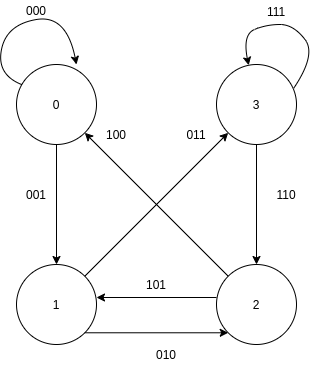
\includegraphics[width=0.3\textwidth]{capitulo1/images/brujin.png}
	\caption{Diagrama de bruijn genérica para ECA(2, 1))}
	\label{fig:bruijn}
\end{figure}
\newpage

\begin{equation}
	M_{R22}=
	\begin{bmatrix}
	0 & 1 & . & .\\
	. & . &  1 & 0\\
	1 & 0 &  . & .\\
	. & . &  0 & 0\\
	\end{bmatrix}
\end{equation}

La matriz de conexión $M$ correspondiente al diagrama de Bruijn de la Figura \ref{fig:bruijn} se define como sigue:

\begin{center}
	\begin{equation}
		 M_{i,j} = 
		\begin{cases}
			1, & \text{if} j \in \{ki, ki+1,...,ki+k-1 (\text{mod} k^{2r})\}\\
			0, & \text{en otro caso}
			
		\end{cases}
	\end{equation}
\end{center}

donde modulo $k^{2r}$ representa el número de vértices y $j$ toma valores de $\{ki, ki+1,...,ki+k-1 (\text{mod} k^{2r})\}$. Por lo tanto ECA$(2, 1)$ es:

\begin{center}
	\begin{equation}
	M_{i,j} = 
	\begin{cases}
	1, & \text{if} j \in \{2i, 2i+1 (\text{mod} 4)\}\\
	0, & \text{en otro caso}
	\label{eq:eca21}
	\end{cases}
	\end{equation}
\end{center}

Con la disposición de estas ecuaciones es posible crear un programa que permita generar la matriz de adyacencia utilizando específicamente \ref{eq:eca21}.

\definecolor{mygray}{rgb}{0.48,0.66,0.59}

%\inputminted[autogobble]{C++}{../brujin.cpp}
\lstset{backgroundcolor=\color{mygray}}
\lstinputlisting[language=c++, firstline = 1, lastline=35]{../brujin.cpp}
Obteniendo como salida la matriz de adyacencia genérica del diagrama de Bruijn para ECA(2, 1).
\lstset{backgroundcolor=\color{white}}
\lstinputlisting[lastline=5]{../output.out}

Para el caso de las etiquetas de cada arista del grafo también es posible realizar un programa y encontrar los traslapes y la conexión de vertices para cada arista.

%code for connections
\lstset{backgroundcolor=\color{mygray}}
\lstinputlisting[language=c++, firstline = 36, lastline=50]{../brujin.cpp}
En la salida podemos encontrar que el vértice 0 hacia el vértice 0 tiene la etiqueta \textbf{000}, el vértice 0 hacia el vértice 1 tiene la etiqueta \textbf{001} y así sucesivamente.
\lstset{backgroundcolor=\color{white}}
\lstinputlisting[firstline=6]{../output.out}
\newpage
Estos resultados son de una máquina genérica de un ECA(2, 1), sin embargo con ligeras modificaciones podemos encontrar las conexiones específicas para las reglas propuestas:
\lstset{backgroundcolor=\color{mygray}}
\lstinputlisting[language=c++, firstline = 53]{../brujin.cpp}
 \hyperlink{https://github.com/QApolo/CS/tree/master/02_Bruijn}{\textbf{Ver código y reporte}}
\newpage
\section{Regla 15}
\lstset{backgroundcolor=\color{white}}
\lstinputlisting[firstline=18, lastline = 34]{../output2.out}

\begin{figure}[h]
	\centering
	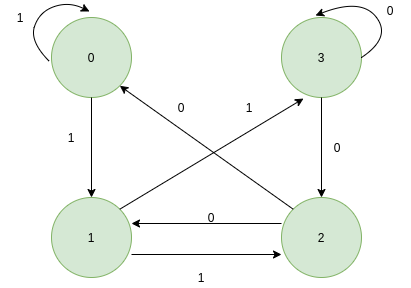
\includegraphics[width=0.5\textwidth]{capitulo1/images/rule15.png}
	\caption{Diagrama de Bruijn regla 15}
	\label{fig:rule15}
\end{figure}

\section{Regla 22}
\lstset{backgroundcolor=\color{white}}
\lstinputlisting[firstline=35, lastline=51]{../output2.out}

\begin{figure}[h]
	\centering
	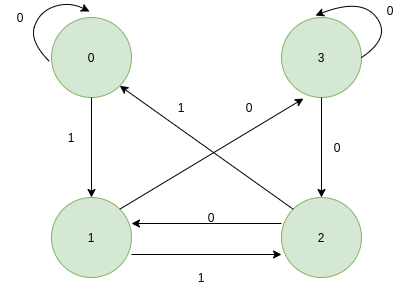
\includegraphics[width=0.5\textwidth]{capitulo1/images/rule22.png}
	\caption{Diagrama de Bruijn regla 22}
	\label{fig:rule22}
\end{figure}

\section{Regla 30}
\lstset{backgroundcolor=\color{white}}
\lstinputlisting[firstline=52, lastline=68]{../output2.out}

\begin{figure}[h]
	\centering
	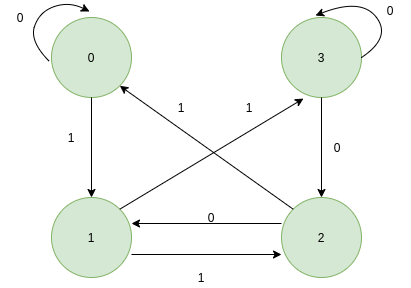
\includegraphics[width=0.5\textwidth]{capitulo1/images/rule30.png}
	\caption{Diagrama de Bruijn regla 30}
	\label{fig:rule30}
\end{figure}
\section{Regla 54}
\lstset{backgroundcolor=\color{white}}
\lstinputlisting[firstline=69, lastline=85]{../output2.out}

\begin{figure}[h]
	\centering
	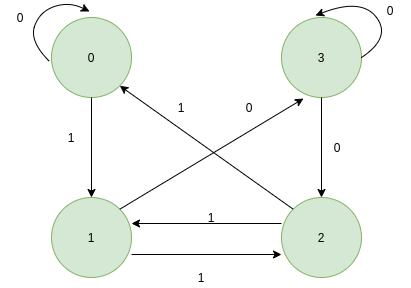
\includegraphics[width=0.5\textwidth]{capitulo1/images/rule54.png}
	\caption{Diagrama de Bruijn regla 54}
	\label{fig:rule54}
\end{figure}
\section{Regla 90}
\lstset{backgroundcolor=\color{white}}
\lstinputlisting[firstline=86, lastline=102]{../output2.out}

\begin{figure}[h]
	\centering
	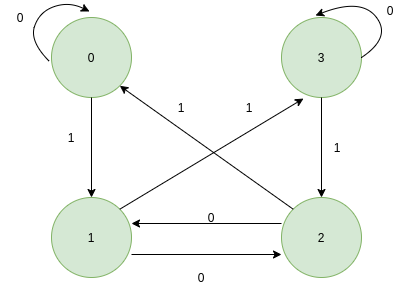
\includegraphics[width=0.5\textwidth]{capitulo1/images/rule90.png}
	\caption{Diagrama de Bruijn regla 90}
	\label{fig:rule90}
\end{figure}


\section{Regla 110}
\lstset{backgroundcolor=\color{white}}
\lstinputlisting[firstline=103]{../output2.out}


\begin{figure}[h]
	\centering
	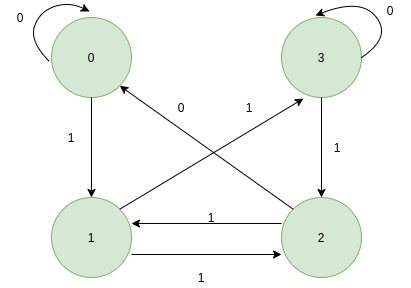
\includegraphics[width=0.5\textwidth]{capitulo1/images/rule110.png}
	\caption{Diagrama de Bruijn regla 110}
	\label{fig:rule110}
\end{figure}